\documentclass{standalone}
\usepackage{tikz}
\usetikzlibrary{patterns, positioning}


\begin{document}
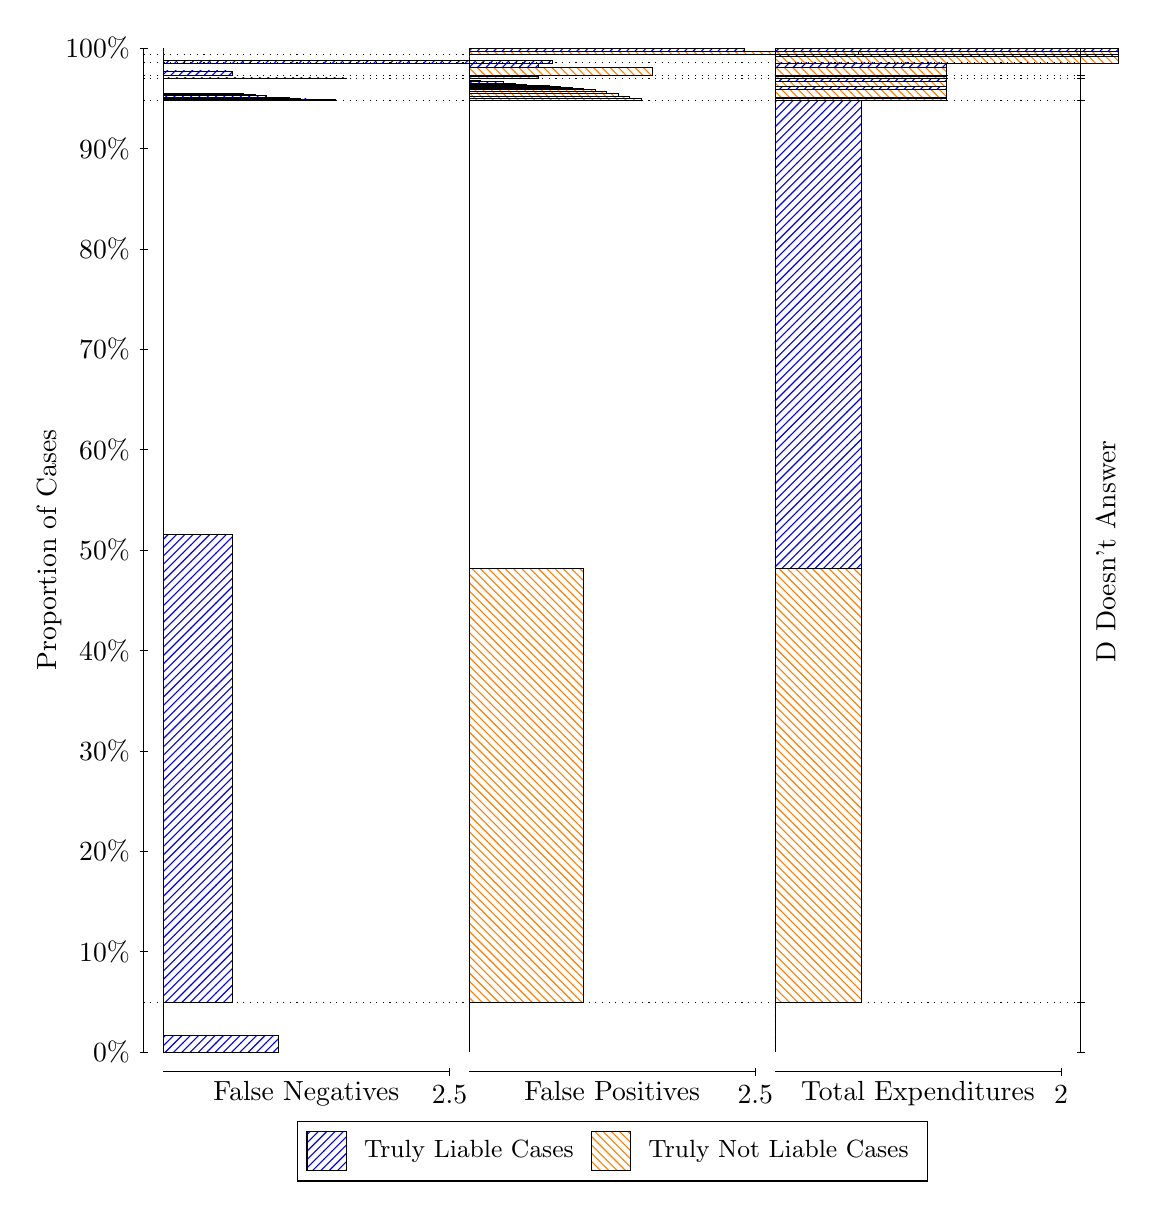
\begin{tikzpicture}
\draw[black, very thin] (1.5,1.75) -- (1.5,14.5);
\node[rotate=90, text=black, anchor=center] at (0.3, 8.125) {Proportion of Cases};
\draw[black, very thin] (1.45,1.75) -- (1.55,1.75);
\node[text=black, anchor=east] at (1.45, 1.75) {0\%};
\draw[black, very thin] (1.45,3.025) -- (1.55,3.025);
\node[text=black, anchor=east] at (1.45, 3.025) {10\%};
\draw[black, very thin] (1.45,4.3) -- (1.55,4.3);
\node[text=black, anchor=east] at (1.45, 4.3) {20\%};
\draw[black, very thin] (1.45,5.575) -- (1.55,5.575);
\node[text=black, anchor=east] at (1.45, 5.575) {30\%};
\draw[black, very thin] (1.45,6.85) -- (1.55,6.85);
\node[text=black, anchor=east] at (1.45, 6.85) {40\%};
\draw[black, very thin] (1.45,8.125) -- (1.55,8.125);
\node[text=black, anchor=east] at (1.45, 8.125) {50\%};
\draw[black, very thin] (1.45,9.4) -- (1.55,9.4);
\node[text=black, anchor=east] at (1.45, 9.4) {60\%};
\draw[black, very thin] (1.45,10.675) -- (1.55,10.675);
\node[text=black, anchor=east] at (1.45, 10.675) {70\%};
\draw[black, very thin] (1.45,11.95) -- (1.55,11.95);
\node[text=black, anchor=east] at (1.45, 11.95) {80\%};
\draw[black, very thin] (1.45,13.225) -- (1.55,13.225);
\node[text=black, anchor=east] at (1.45, 13.225) {90\%};
\draw[black, very thin] (1.45,14.5) -- (1.55,14.5);
\node[text=black, anchor=east] at (1.45, 14.5) {100\%};

\draw[black, very thin] (13.4,1.75) -- (13.4,14.5);
\draw[black, very thin] (13.35,1.75) -- (13.45,1.75);
\node[anchor=west] at (13.35, 1.75) {};
\draw[black, very thin] (13.35,2.3805) -- (13.45,2.3805);
\node[anchor=west] at (13.35, 2.3805) {};
\draw[black, very thin] (13.35,13.837) -- (13.45,13.837);
\node[anchor=west] at (13.35, 13.837) {};
\draw[black, very thin] (13.35,14.113) -- (13.45,14.113);
\node[anchor=west] at (13.35, 14.113) {};
\draw[black, very thin] (13.35,14.148) -- (13.45,14.148);
\node[anchor=west] at (13.35, 14.148) {};
\draw[black, very thin] (13.35,14.312) -- (13.45,14.312);
\node[anchor=west] at (13.35, 14.312) {};
\draw[black, very thin] (13.35,14.419) -- (13.45,14.419);
\node[anchor=west] at (13.35, 14.419) {};
\draw[black, very thin] (13.35,14.5) -- (13.45,14.5);
\node[anchor=west] at (13.35, 14.5) {};

\draw[black, very thin, pattern color=blue, pattern=north east lines] (1.75,1.75) rectangle (3.2033,1.9589);
\draw[black, very thin, pattern color=orange, pattern=north west lines] (1.75,1.9589) rectangle (1.75,2.3805);
\draw[black, very thin, pattern color=blue, pattern=north east lines] (1.75,2.3805) rectangle (2.622,8.3224);
\draw[black, very thin, pattern color=orange, pattern=north west lines] (1.75,8.3224) rectangle (1.75,13.837);
\draw[black, very thin, pattern color=blue, pattern=north east lines] (1.75,13.837) rectangle (3.93,13.844);
\draw[black, very thin, pattern color=blue, pattern=north east lines] (1.75,13.844) rectangle (3.7847,13.848);
\draw[black, very thin, pattern color=blue, pattern=north east lines] (1.75,13.848) rectangle (3.6393,13.854);
\draw[black, very thin, pattern color=blue, pattern=north east lines] (1.75,13.854) rectangle (3.494,13.86);
\draw[black, very thin, pattern color=blue, pattern=north east lines] (1.75,13.86) rectangle (3.3487,13.871);
\draw[black, very thin, pattern color=blue, pattern=north east lines] (1.75,13.871) rectangle (3.2033,13.878);
\draw[black, very thin, pattern color=blue, pattern=north east lines] (1.75,13.878) rectangle (3.058,13.896);
\draw[black, very thin, pattern color=blue, pattern=north east lines] (1.75,13.896) rectangle (2.9127,13.91);
\draw[black, very thin, pattern color=blue, pattern=north east lines] (1.75,13.91) rectangle (2.7673,13.923);
\draw[black, very thin, pattern color=orange, pattern=north west lines] (1.75,13.923) rectangle (1.75,14.113);
\draw[black, very thin, pattern color=blue, pattern=north east lines] (1.75,14.113) rectangle (4.0753,14.12);
\draw[black, very thin, pattern color=orange, pattern=north west lines] (1.75,14.12) rectangle (1.75,14.148);
\draw[black, very thin, pattern color=blue, pattern=north east lines] (1.75,14.148) rectangle (2.622,14.209);
\draw[black, very thin, pattern color=orange, pattern=north west lines] (1.75,14.209) rectangle (1.75,14.312);
\draw[black, very thin, pattern color=blue, pattern=north east lines] (1.75,14.312) rectangle (6.6913,14.341);
\draw[black, very thin, pattern color=orange, pattern=north west lines] (1.75,14.341) rectangle (1.75,14.419);
\draw[black, very thin, pattern color=orange, pattern=north west lines] (1.75,14.419) rectangle (1.75,14.459);
\draw[black, very thin, pattern color=blue, pattern=north east lines] (1.75,14.459) rectangle (1.75,14.5);
\draw[black, very thin, pattern color=orange, pattern=north west lines] (5.6333,1.75) rectangle (5.6333,2.1717);
\draw[black, very thin, pattern color=blue, pattern=north east lines] (5.6333,2.1717) rectangle (5.6333,2.3805);
\draw[black, very thin, pattern color=orange, pattern=north west lines] (5.6333,2.3805) rectangle (7.0867,7.8955);
\draw[black, very thin, pattern color=blue, pattern=north east lines] (5.6333,7.8955) rectangle (5.6333,13.837);
\draw[black, very thin, pattern color=orange, pattern=north west lines] (5.6333,13.837) rectangle (7.8133,13.858);
\draw[black, very thin, pattern color=orange, pattern=north west lines] (5.6333,13.858) rectangle (7.668,13.883);
\draw[black, very thin, pattern color=orange, pattern=north west lines] (5.6333,13.883) rectangle (7.5227,13.924);
\draw[black, very thin, pattern color=orange, pattern=north west lines] (5.6333,13.924) rectangle (7.3773,13.945);
\draw[black, very thin, pattern color=orange, pattern=north west lines] (5.6333,13.945) rectangle (7.232,13.975);
\draw[black, very thin, pattern color=orange, pattern=north west lines] (5.6333,13.975) rectangle (7.0867,13.989);
\draw[black, very thin, pattern color=orange, pattern=north west lines] (5.6333,13.989) rectangle (6.9413,14.004);
\draw[black, very thin, pattern color=orange, pattern=north west lines] (5.6333,14.004) rectangle (6.796,14.013);
\draw[black, very thin, pattern color=orange, pattern=north west lines] (5.6333,14.013) rectangle (6.6507,14.027);
\draw[black, very thin, pattern color=blue, pattern=north east lines] (5.6333,14.027) rectangle (6.36,14.04);
\draw[black, very thin, pattern color=blue, pattern=north east lines] (5.6333,14.04) rectangle (6.2147,14.054);
\draw[black, very thin, pattern color=blue, pattern=north east lines] (5.6333,14.054) rectangle (6.0693,14.072);
\draw[black, very thin, pattern color=blue, pattern=north east lines] (5.6333,14.072) rectangle (5.924,14.079);
\draw[black, very thin, pattern color=blue, pattern=north east lines] (5.6333,14.079) rectangle (5.7787,14.09);
\draw[black, very thin, pattern color=blue, pattern=north east lines] (5.6333,14.09) rectangle (5.6333,14.113);
\draw[black, very thin, pattern color=orange, pattern=north west lines] (5.6333,14.113) rectangle (6.5053,14.14);
\draw[black, very thin, pattern color=blue, pattern=north east lines] (5.6333,14.14) rectangle (5.6333,14.148);
\draw[black, very thin, pattern color=orange, pattern=north west lines] (5.6333,14.148) rectangle (7.9587,14.252);
\draw[black, very thin, pattern color=blue, pattern=north east lines] (5.6333,14.252) rectangle (6.5053,14.312);
\draw[black, very thin, pattern color=orange, pattern=north west lines] (5.6333,14.312) rectangle (5.6333,14.39);
\draw[black, very thin, pattern color=blue, pattern=north east lines] (5.6333,14.39) rectangle (5.6333,14.419);
\draw[black, very thin, pattern color=orange, pattern=north west lines] (5.6333,14.419) rectangle (10.575,14.459);
\draw[black, very thin, pattern color=blue, pattern=north east lines] (5.6333,14.459) rectangle (9.1213,14.5);
\draw[black, very thin, pattern color=orange, pattern=north west lines] (9.5167,1.75) rectangle (9.5167,2.1717);
\draw[black, very thin, pattern color=blue, pattern=north east lines] (9.5167,2.1717) rectangle (9.5167,2.3805);
\draw[black, very thin, pattern color=orange, pattern=north west lines] (9.5167,2.3805) rectangle (10.607,7.8955);
\draw[black, very thin, pattern color=blue, pattern=north east lines] (9.5167,7.8955) rectangle (10.607,13.837);
\draw[black, very thin, pattern color=orange, pattern=north west lines] (9.5167,13.837) rectangle (11.697,13.867);
\draw[black, very thin, pattern color=blue, pattern=north east lines] (9.5167,13.867) rectangle (11.697,13.878);
\draw[black, very thin, pattern color=orange, pattern=north west lines] (9.5167,13.878) rectangle (11.697,13.971);
\draw[black, very thin, pattern color=blue, pattern=north east lines] (9.5167,13.971) rectangle (11.697,14.014);
\draw[black, very thin, pattern color=orange, pattern=north west lines] (9.5167,14.014) rectangle (11.697,14.081);
\draw[black, very thin, pattern color=blue, pattern=north east lines] (9.5167,14.081) rectangle (11.697,14.113);
\draw[black, very thin, pattern color=orange, pattern=north west lines] (9.5167,14.113) rectangle (11.697,14.14);
\draw[black, very thin, pattern color=blue, pattern=north east lines] (9.5167,14.14) rectangle (11.697,14.148);
\draw[black, very thin, pattern color=orange, pattern=north west lines] (9.5167,14.148) rectangle (11.697,14.252);
\draw[black, very thin, pattern color=blue, pattern=north east lines] (9.5167,14.252) rectangle (11.697,14.312);
\draw[black, very thin, pattern color=orange, pattern=north west lines] (9.5167,14.312) rectangle (13.877,14.39);
\draw[black, very thin, pattern color=blue, pattern=north east lines] (9.5167,14.39) rectangle (13.877,14.419);
\draw[black, very thin, pattern color=orange, pattern=north west lines] (9.5167,14.419) rectangle (13.877,14.459);
\draw[black, very thin, pattern color=blue, pattern=north east lines] (9.5167,14.459) rectangle (13.877,14.5);
\draw[black, dotted] (1.5,2.3805) -- (13.4,2.3805);
\draw[black, dotted] (1.5,13.837) -- (13.4,13.837);
\draw[black, dotted] (1.5,14.113) -- (13.4,14.113);
\draw[black, dotted] (1.5,14.148) -- (13.4,14.148);
\draw[black, dotted] (1.5,14.312) -- (13.4,14.312);
\draw[black, dotted] (1.5,14.419) -- (13.4,14.419);
\draw[black, very thin] (1.75,1.5) -- (5.3833,1.5);
\node[text=black, anchor=north] at (3.5667, 1.5) {False Negatives};
\draw[black, very thin] (5.3833,1.45) -- (5.3833,1.55);
\node[text=black, anchor=north] at (5.3833, 1.45) {2.5};

\draw[black, very thin] (5.6333,1.5) -- (9.2667,1.5);
\node[text=black, anchor=north] at (7.45, 1.5) {False Positives};
\draw[black, very thin] (9.2667,1.45) -- (9.2667,1.55);
\node[text=black, anchor=north] at (9.2667, 1.45) {2.5};

\draw[black, very thin] (9.5167,1.5) -- (13.15,1.5);
\node[text=black, anchor=north] at (11.333, 1.5) {Total Expenditures};
\draw[black, very thin] (13.15,1.45) -- (13.15,1.55);
\node[text=black, anchor=north] at (13.15, 1.45) {2};


\node[text=black, centered, rotate=90] at (13.72, 8.1089) {D Doesn't Answer};






\draw (7.449999999999999,1.5) node[draw=none] (baseCoordinate) {};
\begin{scope}[align=center]
        \matrix[scale=0.5, draw=black, below=0.5cm of baseCoordinate, nodes={draw}, column sep=0.1cm]{
            \node[rectangle, draw, minimum width=0.5cm, minimum height=0.5cm, pattern color=blue, pattern=north east lines] {}; &
            \node[draw=none, font=\small, text=black] (B) {Truly Liable Cases}; &
            \node[rectangle, draw, minimum width=0.5cm, minimum height=0.5cm, pattern color=orange, pattern=north west lines] {}; &
            \node[draw=none, font=\small, text=black] (B) {Truly Not Liable Cases}; \\
            };
\end{scope}

\end{tikzpicture}
\end{document}